\documentclass[journal,12pt,twocolumn]{IEEEtran}
\usepackage{tkz-euclide} % loads TikZ and tkz-base
\usepackage{hyperref}
\usepackage{xcolor}
\title{AI1110 Software Project Report}
\author{K.SaiTeja\\ (AI22BTECH11014)}
\date{\today}

\begin{document}
\maketitle

\section{Introduction}
The objective of this project is to develop a simple audio player using Python and the Pygame library. The audio player allows users to play a collection of MP3 files stored in a specified directory. It offers basic playback controls such as play, pause, resume, next, and quit. Additionally, the order of the audio files is shuffled to provide variation during playback.

\section{Implementation}
The project implementation can be summarized as follows:

\subsection{Importing Required Libraries}
The necessary libraries, including \texttt{os}, \texttt{numpy}, and \texttt{pygame}, are imported to enable file operations, shuffling, and audio playback, respectively.
\begin{figure}[h]
    \centering
    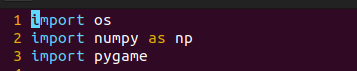
\includegraphics[width = 0.4\textwidth]{figs/fig1.png}
    \caption{Playing songs randomly}
    \label{fig:my_label}
\end{figure}

\subsection{Setting the Audio Directory}
The audio directory path is specified, which represents the location where the MP3 files are stored.
\begin{figure}[h]
    \centering
    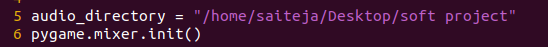
\includegraphics[width = 0.4\textwidth]{figs/fig2.png}
    \caption{Audio Directory and Python Mixer} 
    \label{fig:my_label}
\end{figure}

\subsection{Initializing Pygame Mixer}
The Pygame mixer module is initialized to enable audio playback functionality.

\subsection{Creating a List of Audio Files}
The program retrieves a list of files in the audio directory using \texttt{os.listdir}, filters for MP3 files using the \texttt{.endswith(".mp3")} condition, and creates a list containing the full paths to these audio files.

\subsection{Iterating Through the Audio Files}
The program loops through the audio files. Before each iteration, the list of audio files is shuffled using \texttt{np.random.shuffle} to randomize the order.

\subsection{Audio Playback}
For each audio file, it is loaded using \texttt{pygame.mixer.music.load} and played using \texttt{pygame.mixer.music.play}. The name of the currently playing song is displayed.

\subsection{User Interaction}
While the audio is playing or paused, the program waits for user input. The user can enter commands such as "1" to pause, "2" to resume, "3" to skip to the next song, or "4" to quit the application. The program responds accordingly to the user's commands by invoking the appropriate Pygame mixer functions.
\begin{figure}[h]
    \centering
    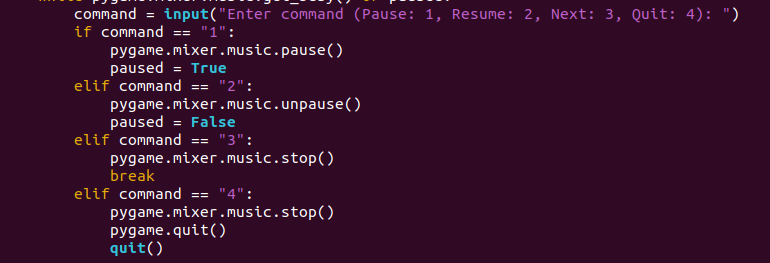
\includegraphics[width = 0.4\textwidth]{figs/fig3.png}
    \caption{User Inputs}
    \label{fig:my_label}
\end{figure}

\subsection{Shuffling the Audio Files}
After playing through the entire playlist, the program shuffles the list of audio files again using \texttt{np.random.shuffle} to provide a different order for the next iteration.
\begin{figure}[h]
    \centering
    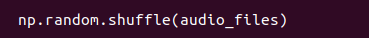
\includegraphics[width = 0.4\textwidth]{figs/fig4.png}
    \caption{Shuffling Playlist}
    \label{fig:my_label}
\end{figure}
\section{Conclusion}
In conclusion, the developed audio player project allows users to play a collection of MP3 files from a specified directory. It provides basic playback controls and shuffles the order of the songs for variation. This project demonstrates the use of Python and the Pygame library to create a simple yet functional audio player. Further enhancements can be made to include features like volume control, playlist management, and graphical user interface (GUI) integration.
\begin{figure}[h]
    \centering
    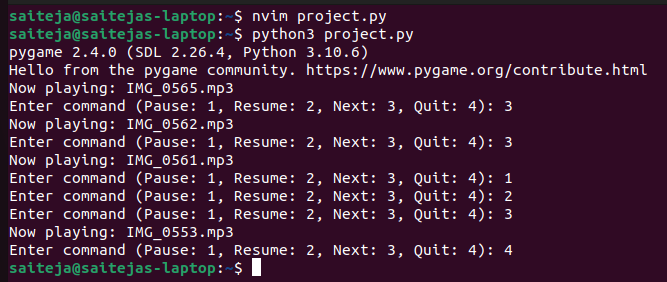
\includegraphics[width = 1\textwidth]{figs/fig5.png}
    \caption{Overall Output Interface}
    \label{fig:my_label}
\end{figure}
\end{document}

